\documentclass{article}
\usepackage[utf8]{inputenc}

\title{Laboratorio 5: Informe sobre el funcionamiento físico de STP y VLAN}
\author{Patricio Inostroza y Matias Castro }
\date{Mayo 2017}

\usepackage{natbib}
\usepackage{graphicx}

\begin{document}

\begin{titlepage}

\maketitle
\huge


\end{titlepage}

\tableofcontents 
\cleardoublepage

\section{Introducción}
En el presente informe se verá y analizará el funcionamiento del protocolo STP y su comportamiento dadas circunstancias específicas a la hora del comienzo del tráfico de información, cómo activar o desactivar este protocolo y cómo crear vlan a través de Putty y un Switch de la marca 3COM, un programa computacional para guiar el funcionamiento de este último. Además, implementaremos distintas VLAN y comprobaremos su funcionamiento con los puertos Trunk y Access. Finalmente resolveremos dudas que pueden darse dado esto.

\newpage

\section{Desarrollo}
\subsection{STP}
El protocolo STP se encarga de determinar cual es la mejor ruta que debe seguir un paquete entre switchs para evitar que se genere un bucle entre enlaces que pueden ser redundantes, fisicamente se utilizara un switch y Putty para manejarlo, con una serie de comandos, primero reiniciando el servidor(reboot) y desactivar el protocolo STP (Figura 1).

\begin{figure}[h!]
\centering
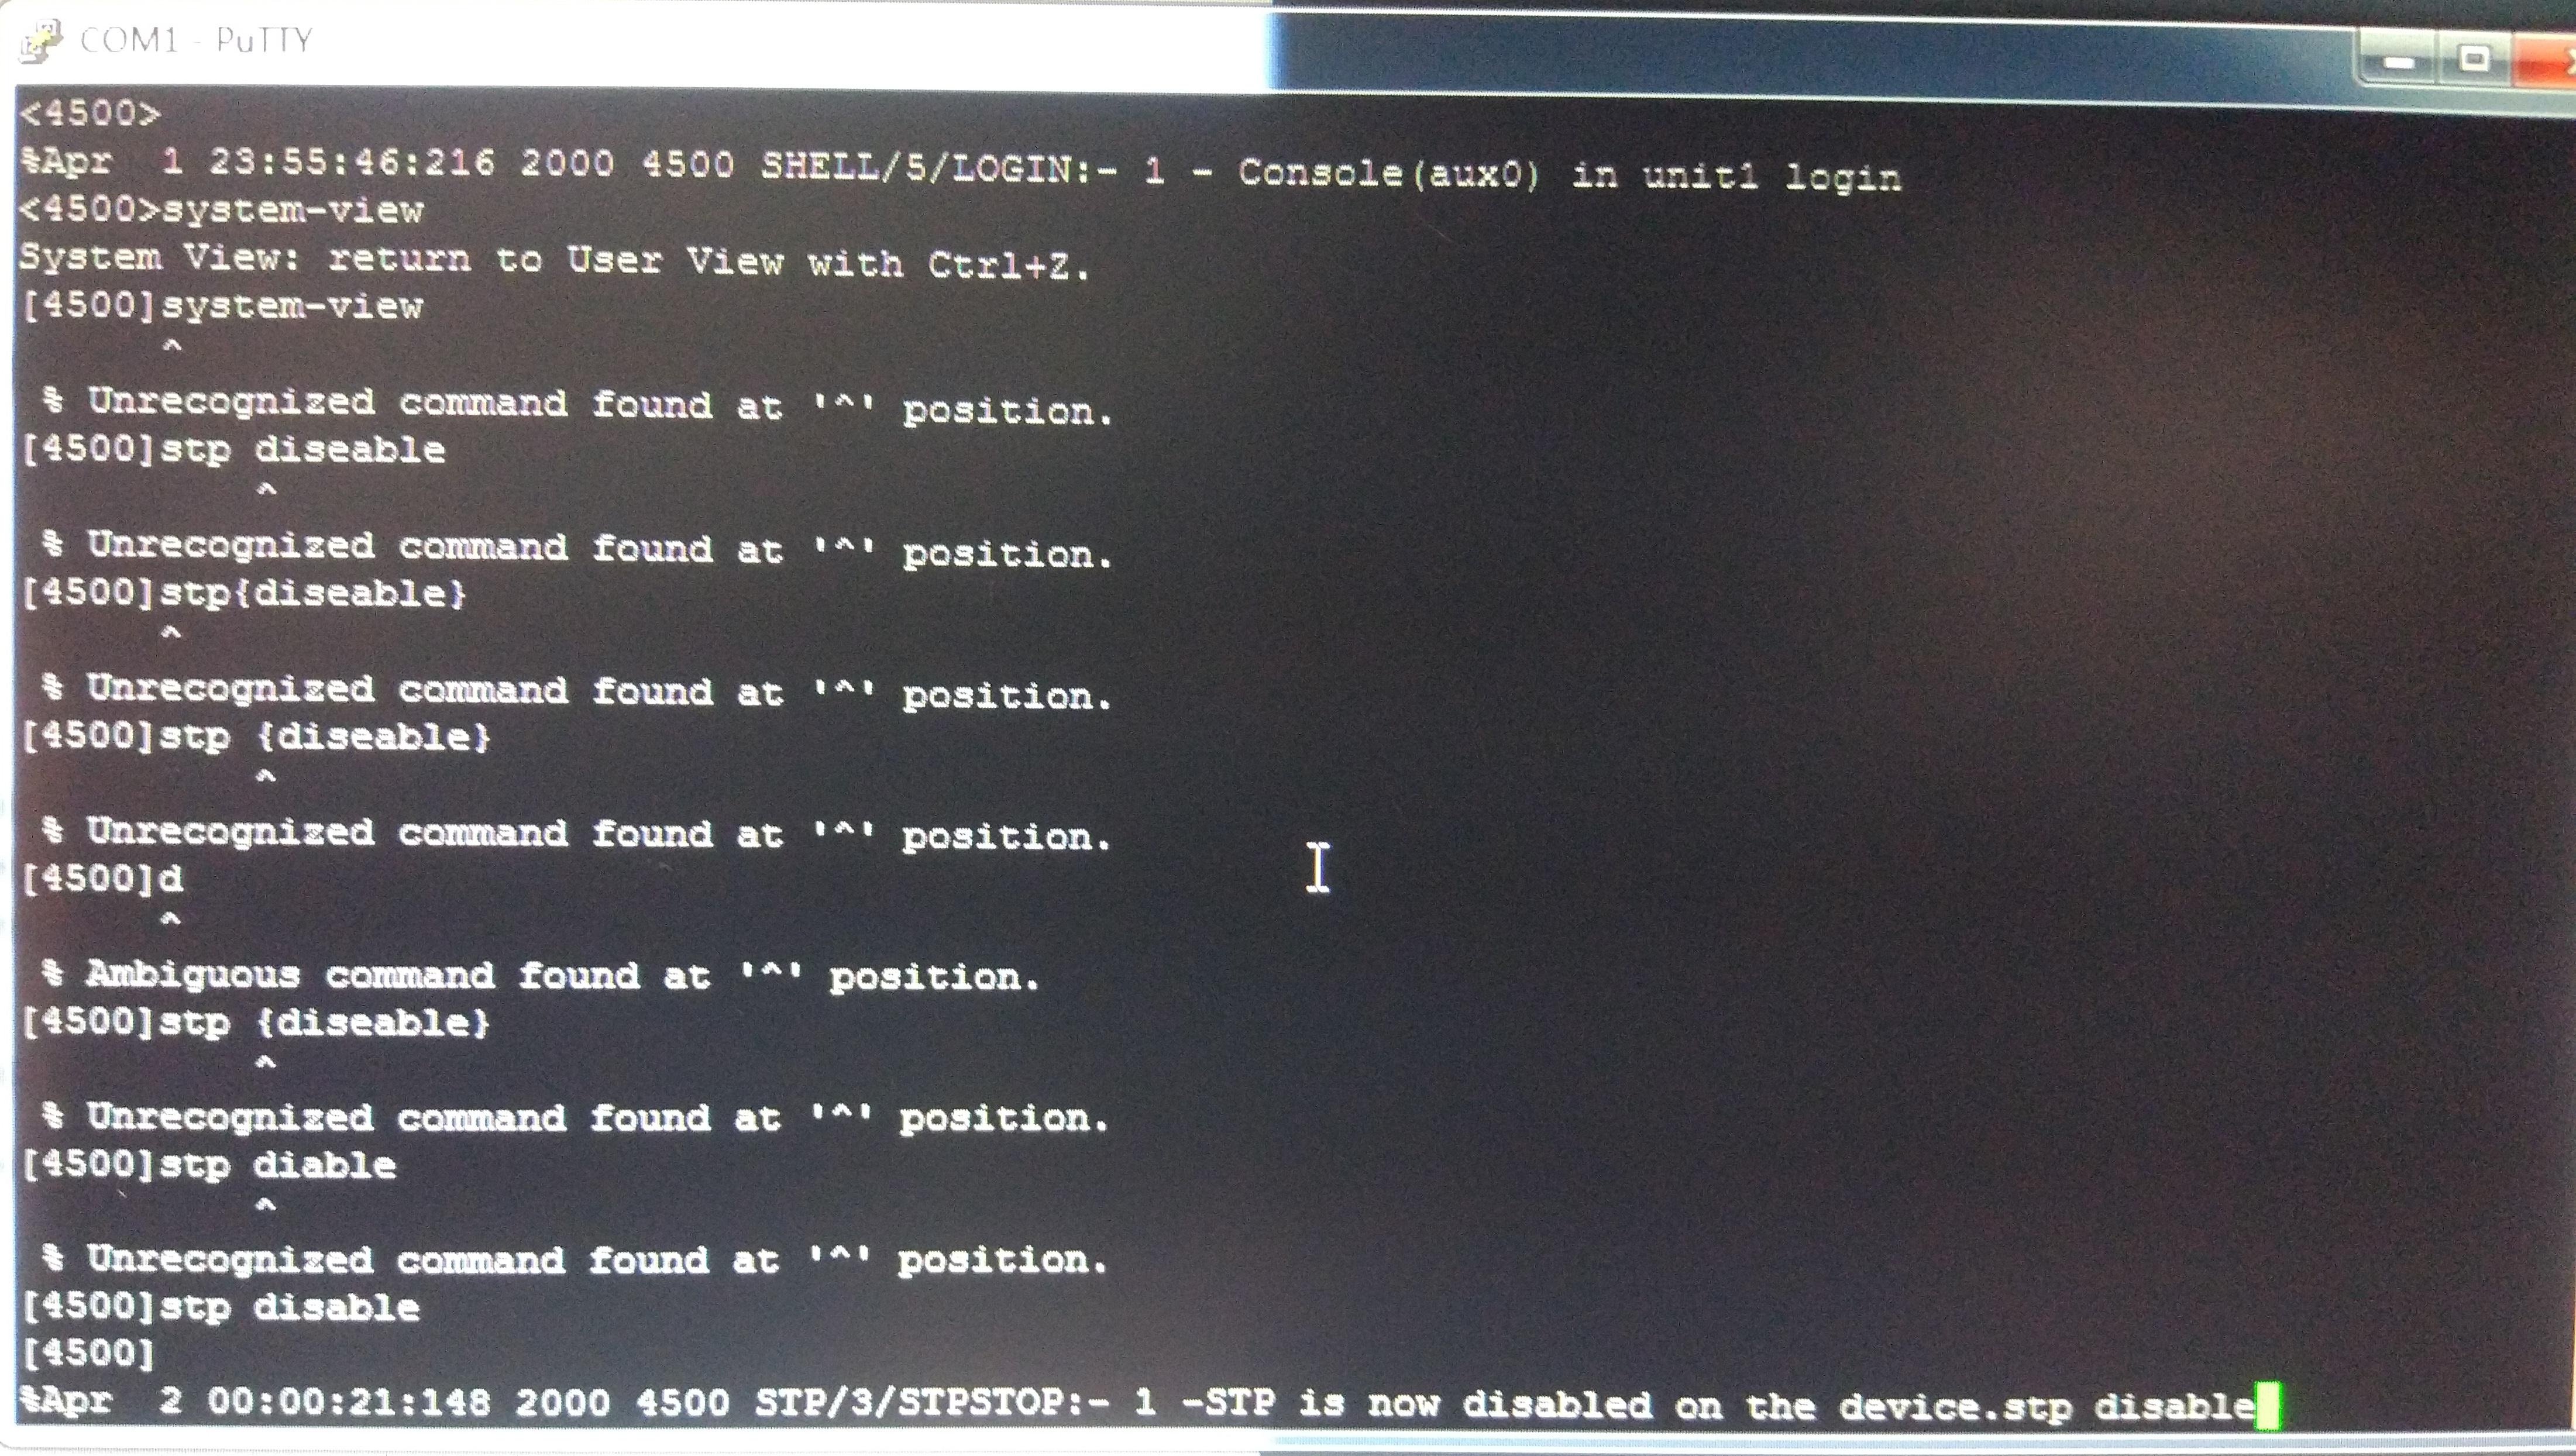
\includegraphics[scale=0.08]{IMG1}
\caption{STP}
\end{figure}

Al momento de hacer esto no se ve ningun problema, pero al conectar un cable utp a otro equipo y hacer ping, las luces de los puertos comienzan a parpadear rapidamente (figura 2), esto significa una tormenta broadcast, al momento de desactivar el STP no se buscó el mejor camino y se generó un bucle, demostrado en el parpadeo.

\begin{figure}[h!]
\centering
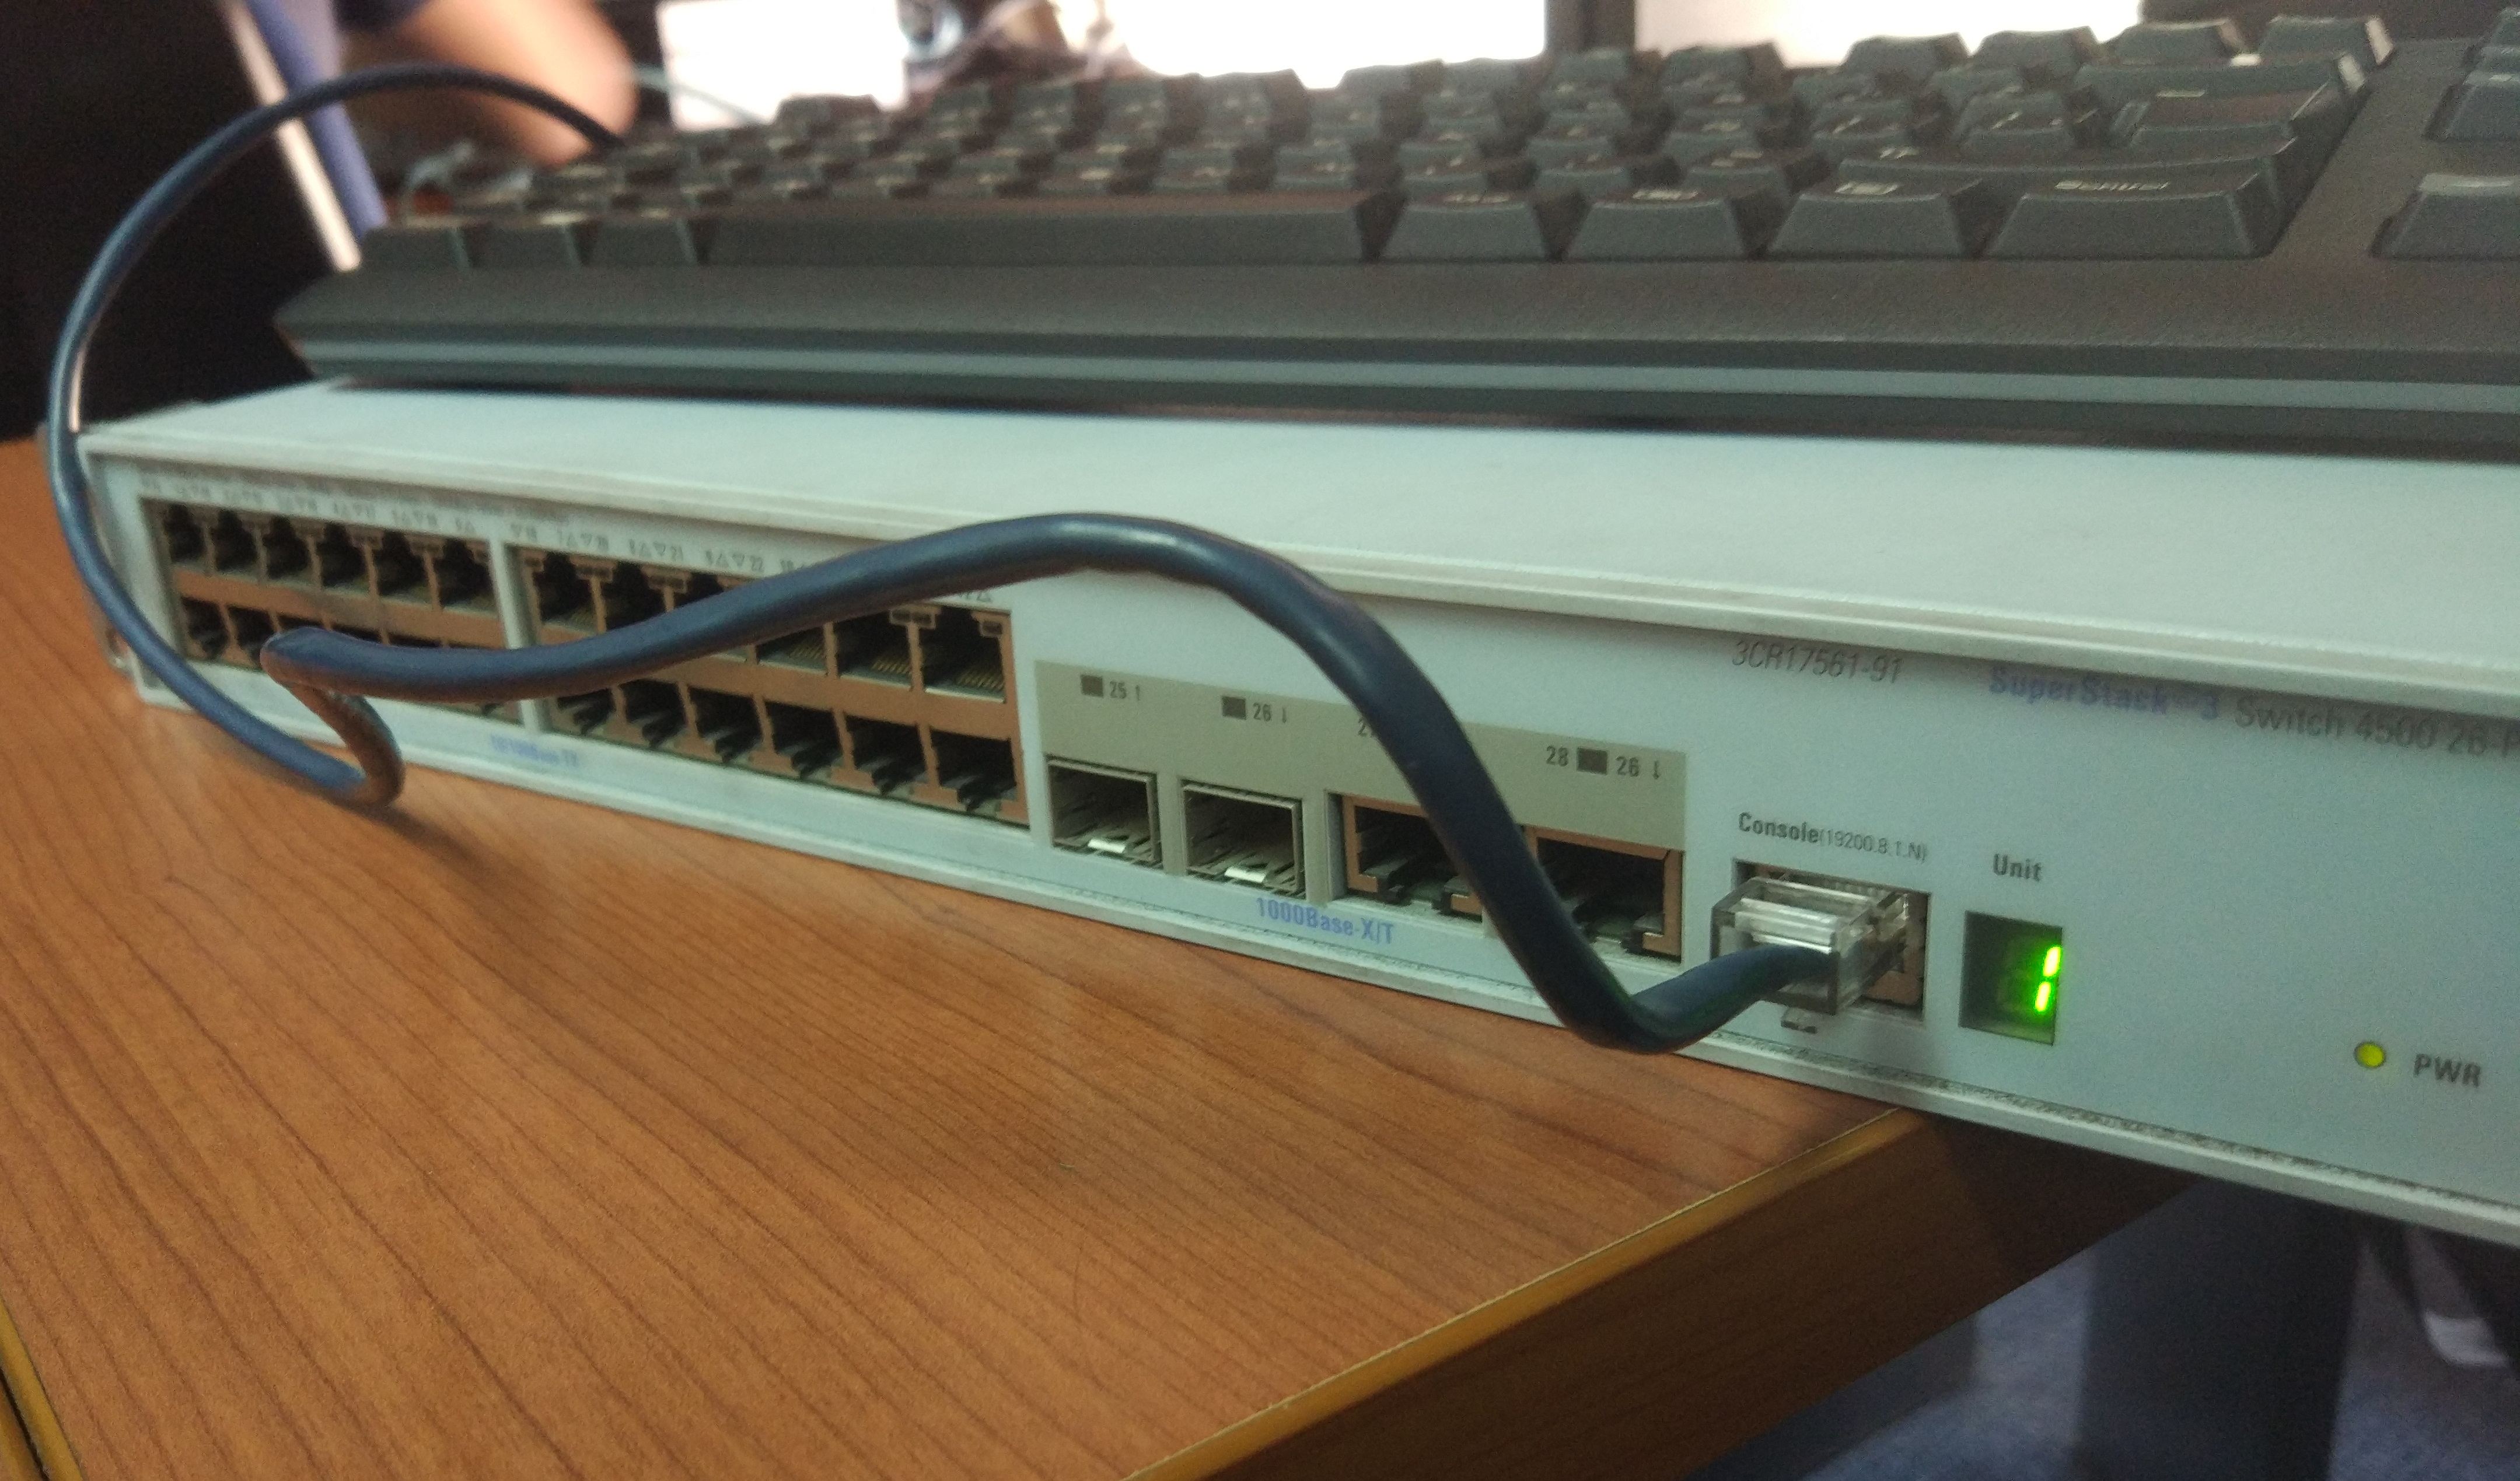
\includegraphics[scale=0.08]{IMG2}
\caption{Switch}
\end{figure}

\subsection{VLAN}

Ahora, por otra parte se ve el funcionamiento de las VLAN, una red local, tambien a través de Putty, creando estas por comandos y estableciendo los puertos del switch como access (del 1 al 6) y uno trunk (el 7) tal como se ve en la figura 3. Luego de introducir correctamente los comandos al hacer ping dentro de la misma LAN se observa el resultado. (figura 4)

\begin{figure}[h!]
\centering
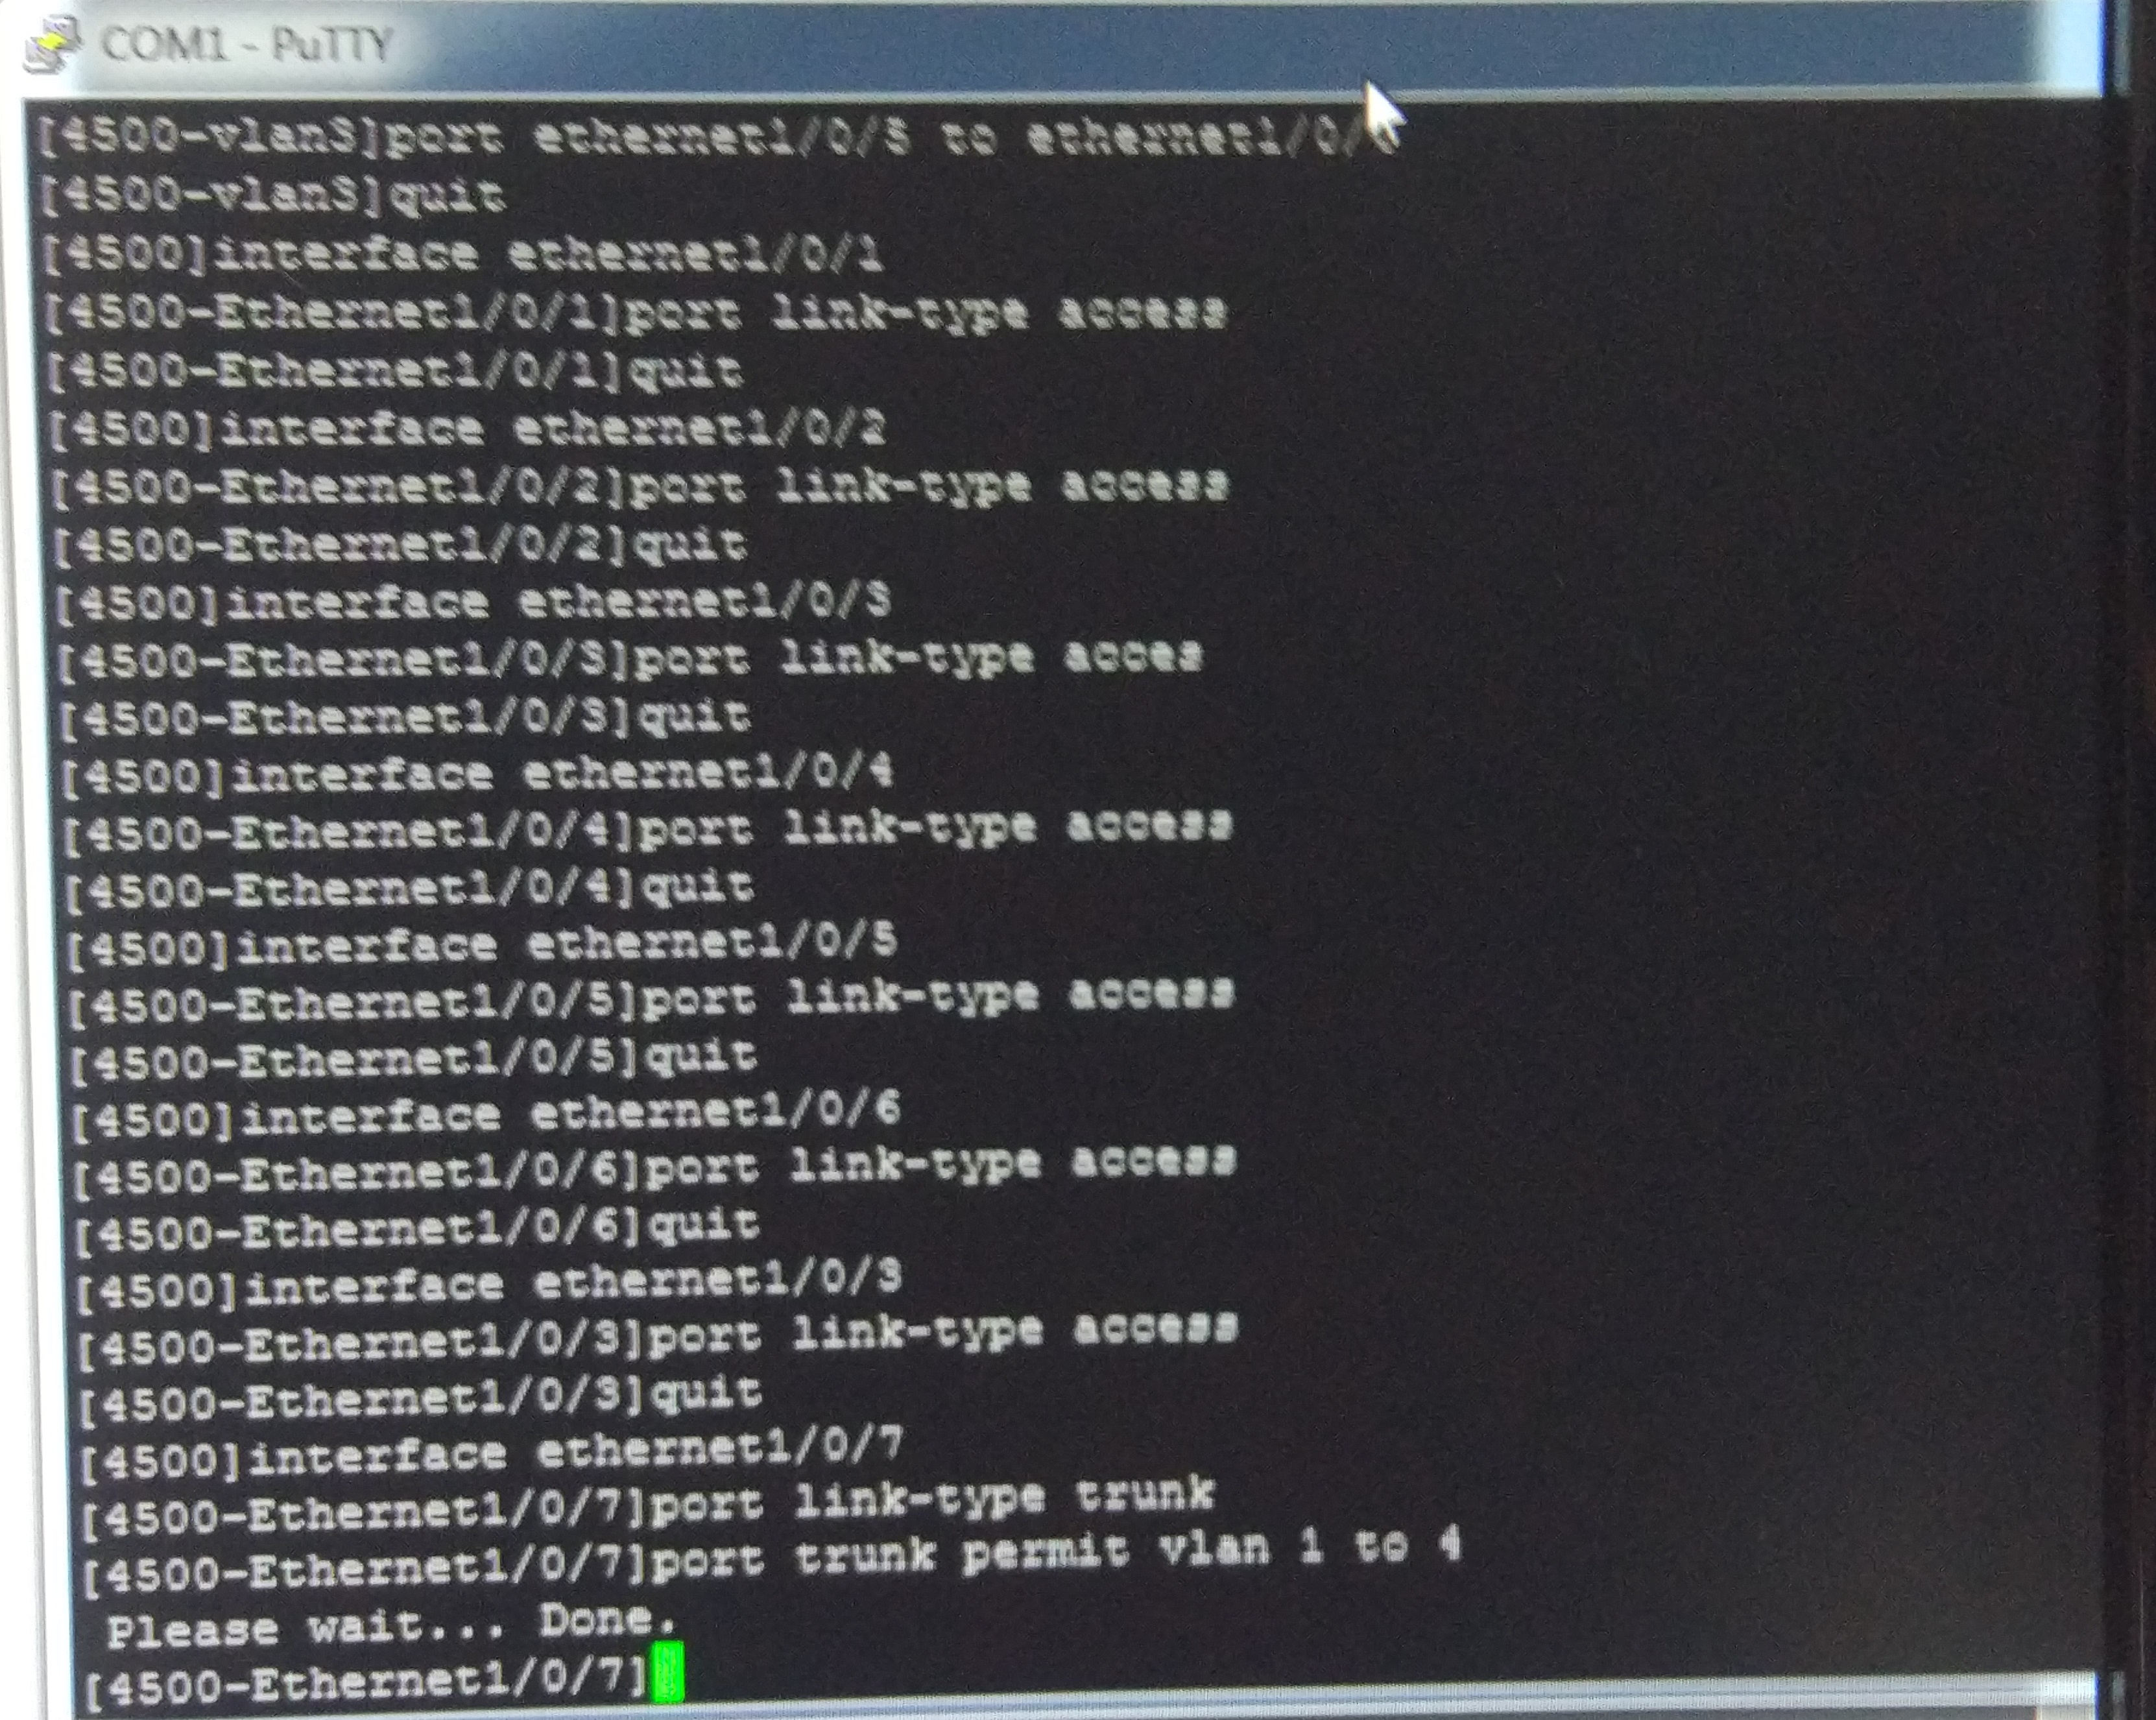
\includegraphics[scale=0.08]{IMG3}
\caption{VLAN}
\end{figure}

\begin{figure}[h!]
\centering
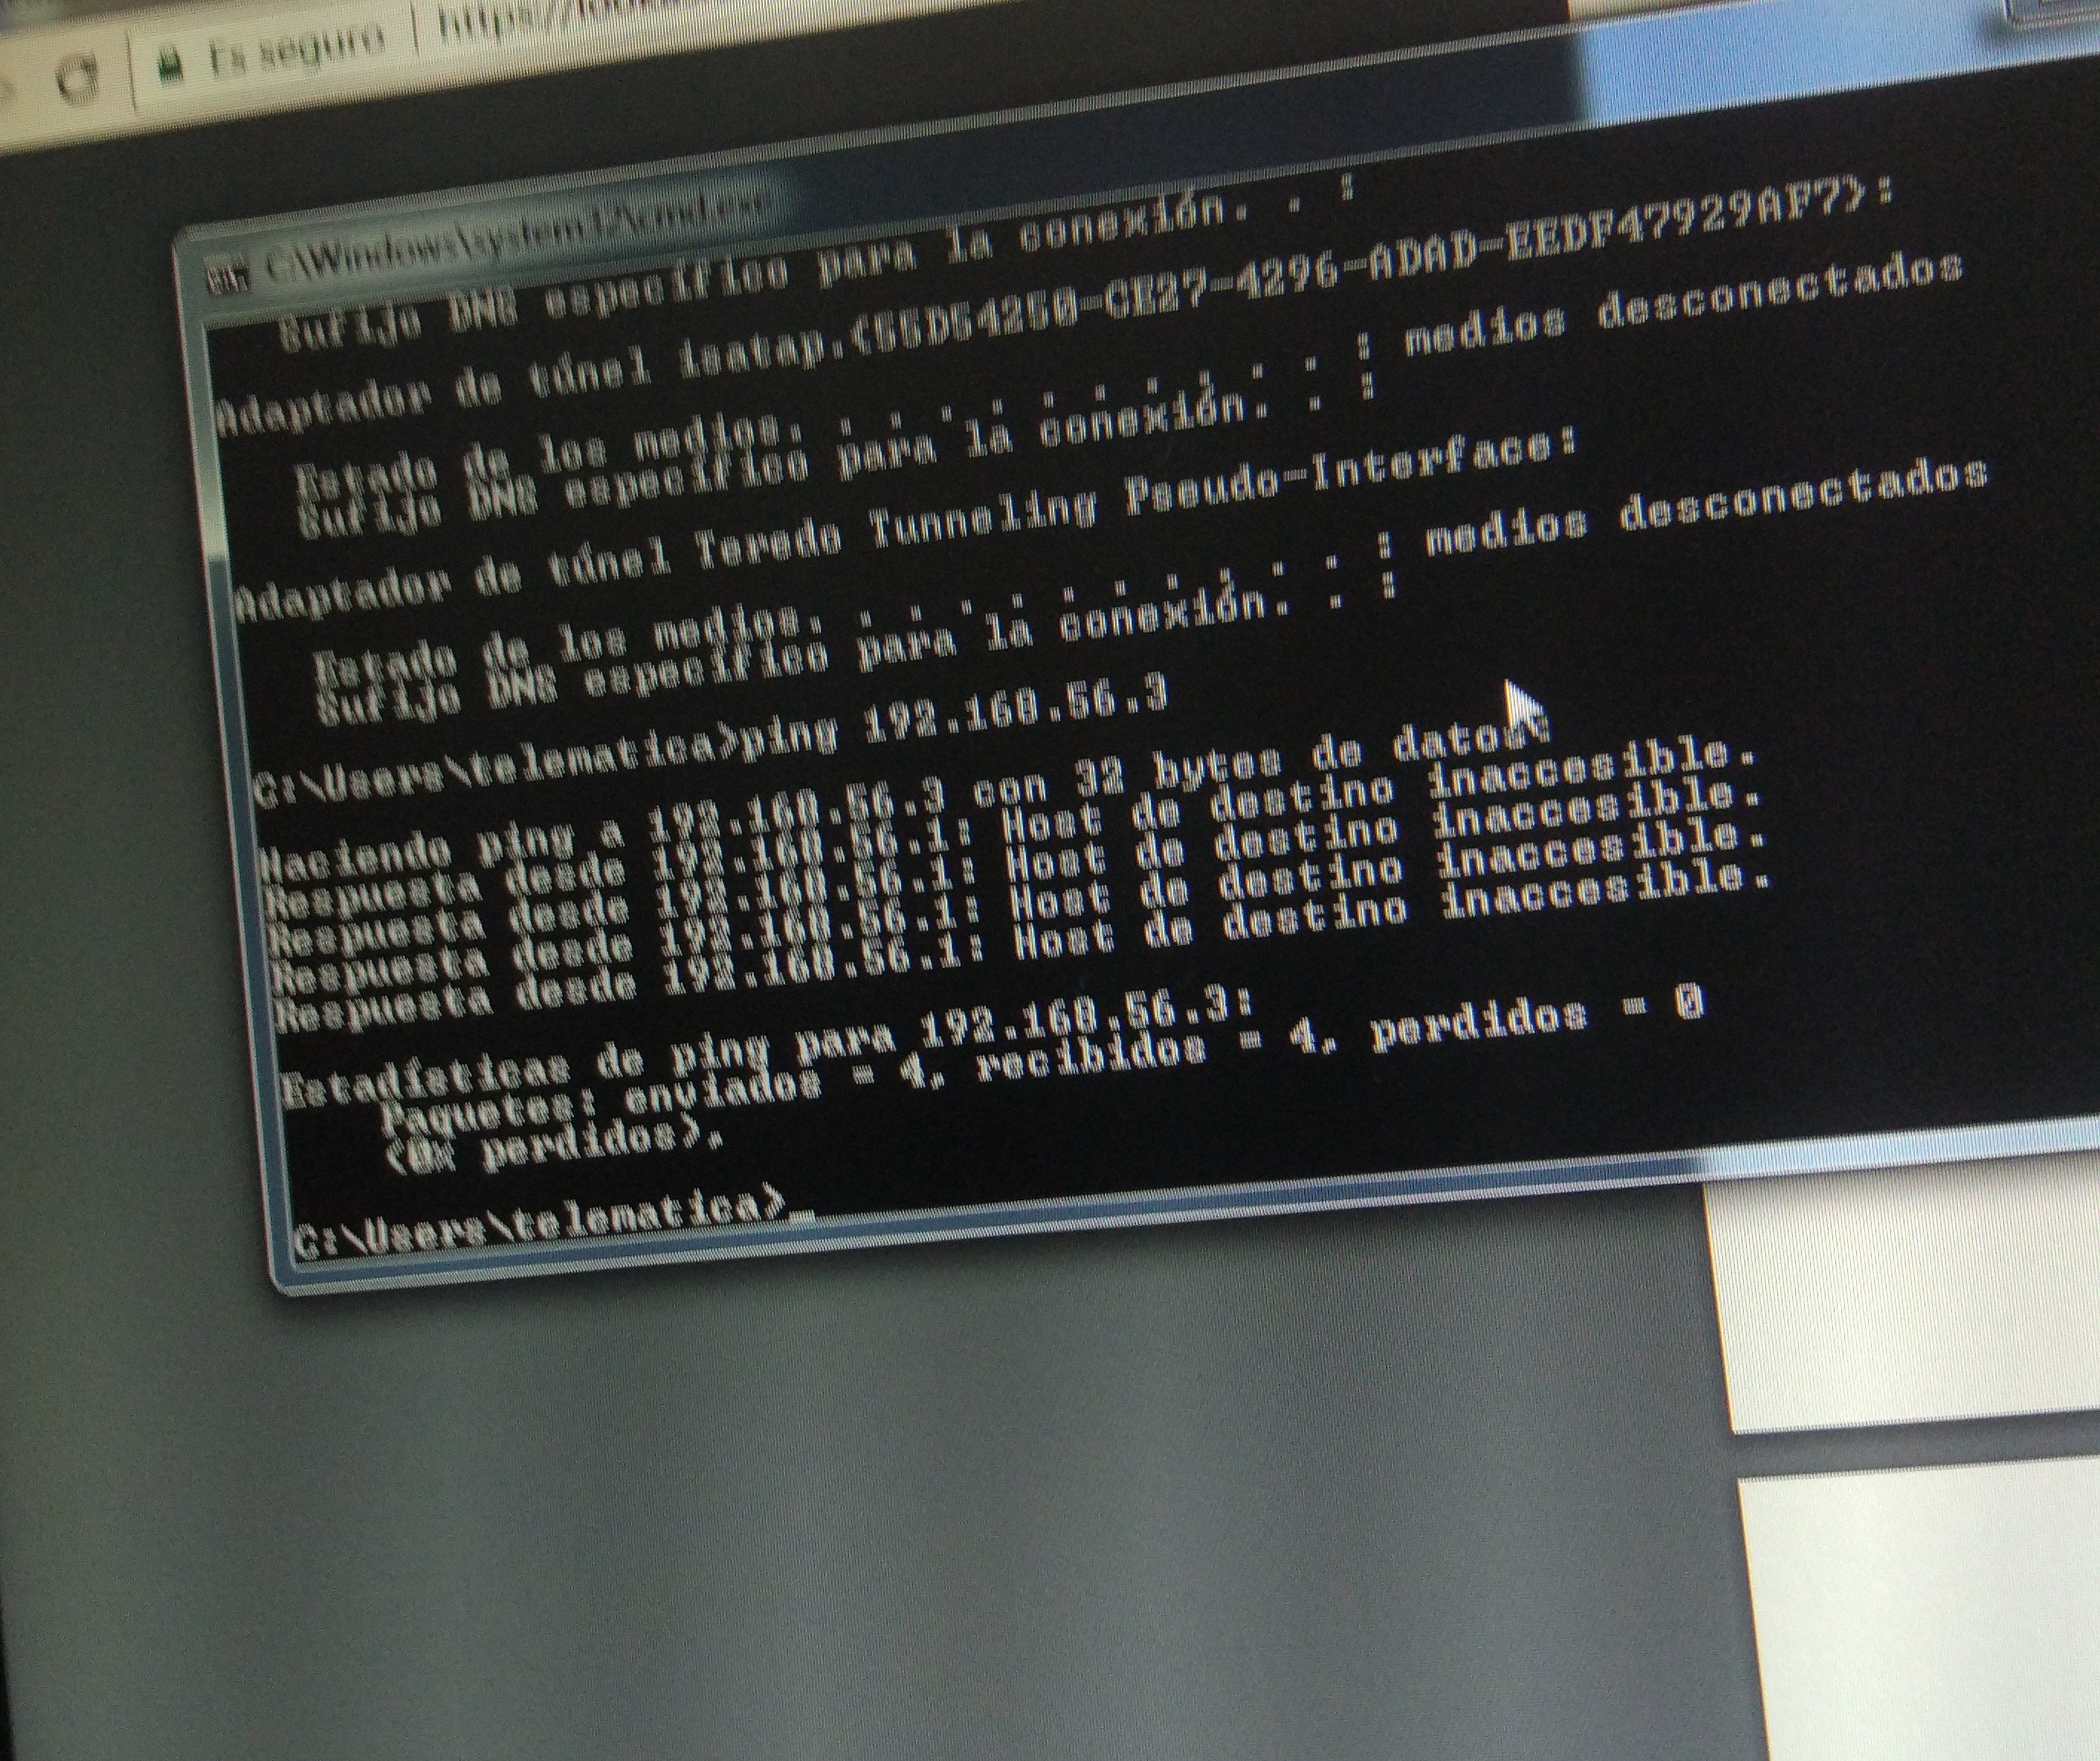
\includegraphics[scale=0.12]{IMG4}
\caption{VLAN}
\end{figure}

\newpage

\section{Preguntas}
1.	¿Qué es y que hace VLAN? Explique 
Es una red local que agrupa un número determinado de equipos, esto virtualmente, ya que no se ve de una manera física, hace segmentación, mejorando el rendimiento de nuestra red. (Smerlin, 2015).\par
2.	¿Qué es y que hace el protocolo STP? Explique. 
Este es un protocolo que se encarga de determinar cuál es la mejor ruta que debe seguir un paquete de información para evitar que se genere un bucle entre enlaces. Si no existe, se genera, por ejemplo, una tormenta broadcast.\par
3.	¿Qué es Putty y para qué sirve? Explique. 
Es un programa con el que podemos conectarnos a servidores remotos (herramientas de una red), controlándolos a través de comandos, para hacer lo que estimemos conveniente. (Alvarez, 2006).\par
4.	Asumiendo que Putty es una herramienta universal, ¿Cuál es la herramienta exclusiva para Linux y Windows que puede hacer lo mismo que Putty? Menciónelas y en el caso de haber investigado ponga el link de donde lo investigo. 
Mobaxterm y Kitty exclusivo para Windows.
https://tecadmin.net/top-5-ssh-clients-for-windows-alternatives-of-putty/ \par
5.	¿Cuáles son las ventajas de haber trabajado primero en Cisco Packet Tracer y luego haber elaborado todo en físico? Mencione y explique al menos 3 aspectos.
Como en todo aspecto, siempre es bueno trabajar primero en lo teórico, y así disminuir los errores a la hora de lo práctico. También packet tracer da herramientas para ver lo que pasa de forma pausada y no a tiempo real que es imposible al trabajar en milisegundos, ver como viaja la información.

\newpage

\section{Conclusión}
El trabajo práctico que se realizó en la configuración del switch era el ultimo paso para entender el funcionamiento y uso del STP (como la tormenta de broadcast que se genera al desactivarlo) y de la creación de redes VLAN y la configuración de sus respectivos puertos (Access o Trunk), tambien la utilización de Putty.

\newpage

\section{Bibliografía}
Alvarez, M. (Julio de 2006). Desarrollo Web. Obtenido de https://desarrolloweb.com/articulos/putty.html
Smerlin, O. (Julio de 2015). Redes y configuración. Obtenido de http://redesconfiguracion.blogspot.cl/2015/07/que-es-una-vlan-y-su-funcion.html


\end{document}
